\documentclass[tikz,border=12pt]{standalone}
\usepackage[T1]{fontenc}
\usepackage{mathpazo}
\usepackage{amsmath,amssymb}
\usetikzlibrary{arrows.meta, positioning, calc, fit, decorations.pathreplacing}

\definecolor{stblue}{HTML}{7B97AD}
\definecolor{rwgold}{HTML}{B8995E}
\definecolor{sage}{HTML}{7A9A7E}
\definecolor{dkbrown}{HTML}{3D3530}
\definecolor{wmgray}{HTML}{7B7067}
\definecolor{cream}{HTML}{F9F6F0}
\definecolor{border}{HTML}{D4C9B8}
\definecolor{terracotta}{HTML}{C47A6A}
\definecolor{lavender}{HTML}{907EA0}

\begin{document}
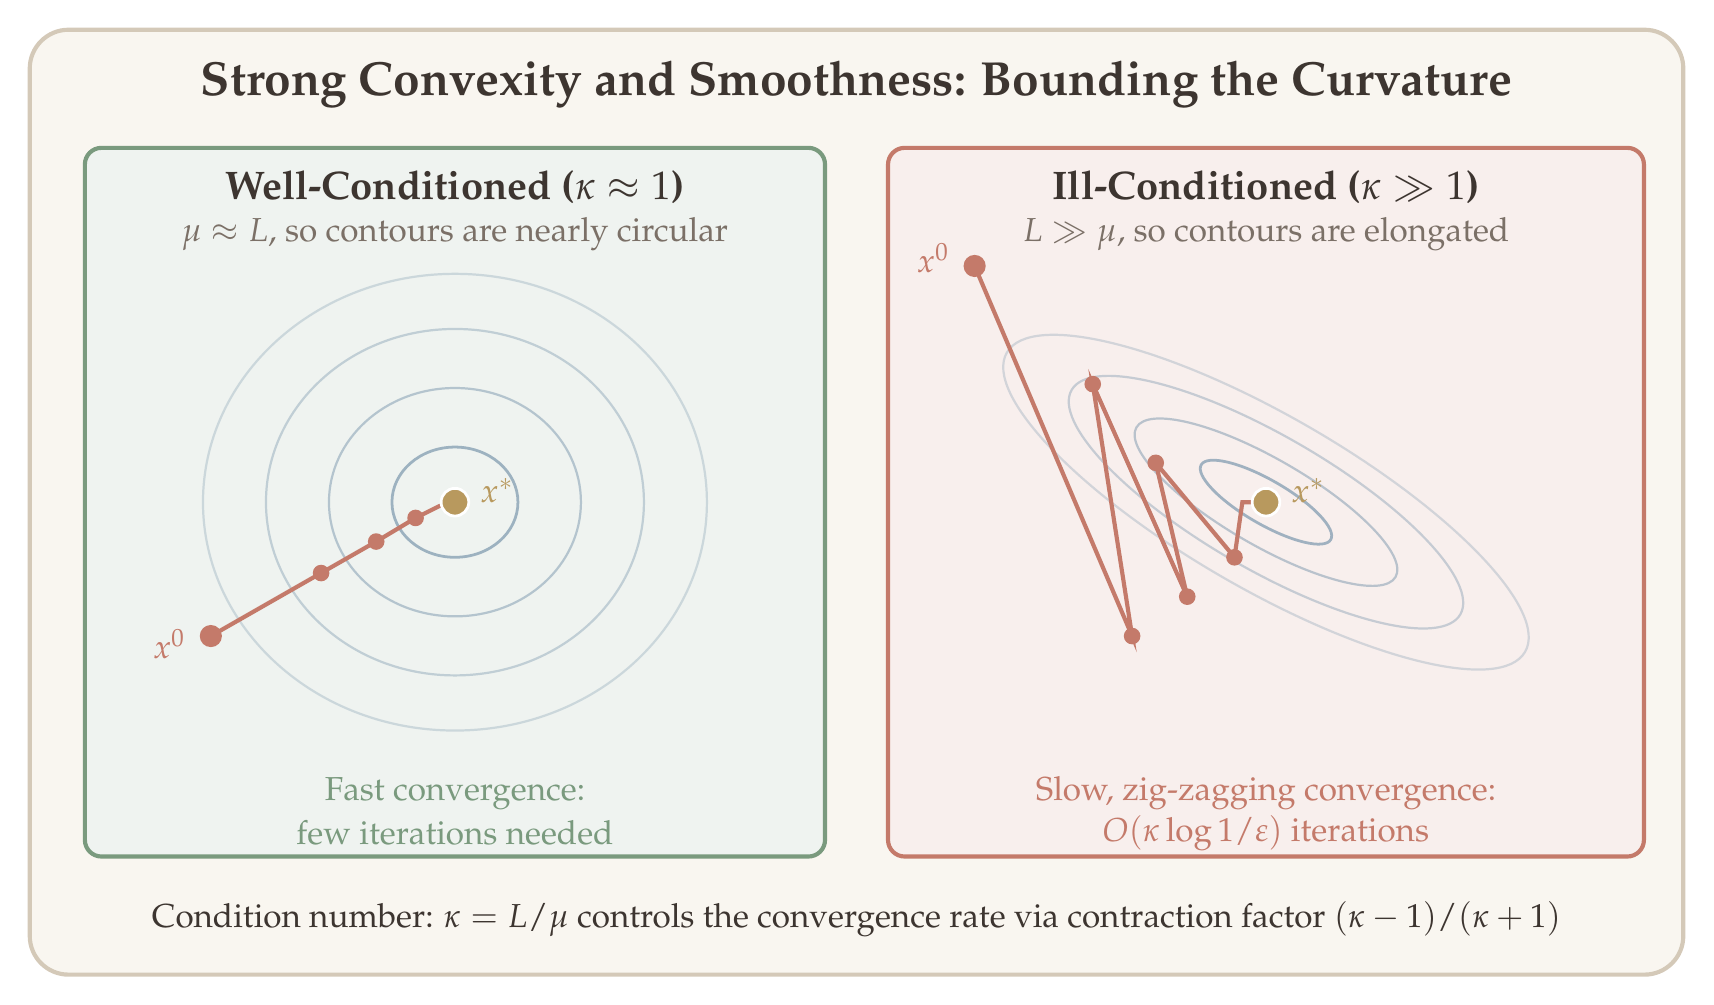
\begin{tikzpicture}[>={Stealth[length=4mm, width=3mm]}]

% Background
\fill[cream, rounded corners=14pt] (-0.5,-0.5) rectangle (20.5,11.5);
\draw[border, line width=1.5pt, rounded corners=14pt] (-0.5,-0.5) rectangle (20.5,11.5);

% Title
\node[text=dkbrown, font=\LARGE\bfseries] at (10,10.8) {Strong Convexity and Smoothness: Bounding the Curvature};

% Left panel: Well-conditioned
\fill[sage!12, rounded corners=6pt] (0.2,1.0) rectangle (9.6,10.0);
\draw[sage, line width=1.5pt, rounded corners=6pt] (0.2,1.0) rectangle (9.6,10.0);

\node[text=dkbrown, font=\Large\bfseries] at (4.9,9.5) {Well-Conditioned ($\kappa \approx 1$)};
\node[text=wmgray, font=\large] at (4.9,8.9) {$\mu \approx L$, so contours are nearly circular};

% Nearly circular contours
\draw[stblue, line width=0.8pt, opacity=0.3] (4.9,5.5) ellipse (3.2 and 2.9);
\draw[stblue, line width=0.8pt, opacity=0.4] (4.9,5.5) ellipse (2.4 and 2.2);
\draw[stblue, line width=0.8pt, opacity=0.5] (4.9,5.5) ellipse (1.6 and 1.45);
\draw[stblue, line width=1pt, opacity=0.7] (4.9,5.5) ellipse (0.8 and 0.7);

% GD trajectory (nearly straight)
\draw[terracotta, line width=1.5pt] (1.8,3.8) -- (3.2,4.6) -- (3.9,5.0) -- (4.4,5.3) -- (4.7,5.45) -- (4.9,5.5);
\fill[terracotta] (1.8,3.8) circle (4pt);
\fill[terracotta] (3.2,4.6) circle (3pt);
\fill[terracotta] (3.9,5.0) circle (3pt);
\fill[terracotta] (4.4,5.3) circle (3pt);
\fill[rwgold] (4.9,5.5) circle (5pt);
\draw[white, line width=1pt] (4.9,5.5) circle (5pt);
\node[text=rwgold, font=\large\bfseries, right] at (5.1,5.65) {$x^*$};
\node[text=terracotta, font=\large, left] at (1.6,3.7) {$x^0$};

\node[text=sage, font=\large] at (4.9,1.8) {Fast convergence:};
\node[text=sage, font=\large] at (4.9,1.3) {few iterations needed};

% Right panel: Ill-conditioned
\fill[terracotta!12, rounded corners=6pt] (10.4,1.0) rectangle (20.0,10.0);
\draw[terracotta, line width=1.5pt, rounded corners=6pt] (10.4,1.0) rectangle (20.0,10.0);

\node[text=dkbrown, font=\Large\bfseries] at (15.2,9.5) {Ill-Conditioned ($\kappa \gg 1$)};
\node[text=wmgray, font=\large] at (15.2,8.9) {$L \gg \mu$, so contours are elongated};

% Elongated ellipses (rotated)
\begin{scope}[rotate around={-30:(15.2,5.5)}]
  \draw[stblue, line width=0.8pt, opacity=0.3] (15.2,5.5) ellipse (3.8 and 1.1);
  \draw[stblue, line width=0.8pt, opacity=0.4] (15.2,5.5) ellipse (2.85 and 0.85);
  \draw[stblue, line width=0.8pt, opacity=0.5] (15.2,5.5) ellipse (1.9 and 0.55);
  \draw[stblue, line width=1pt, opacity=0.7] (15.2,5.5) ellipse (0.95 and 0.28);
\end{scope}

% GD trajectory (zig-zag)
\draw[terracotta, line width=1.5pt] (11.5,8.5) -- (13.5,3.8) -- (13.0,7.0) -- (14.2,4.3) -- (13.8,6.0) -- (14.8,4.8) -- (14.9,5.5) -- (15.2,5.5);
\fill[terracotta] (11.5,8.5) circle (4pt);
\fill[terracotta] (13.5,3.8) circle (3pt);
\fill[terracotta] (13.0,7.0) circle (3pt);
\fill[terracotta] (14.2,4.3) circle (3pt);
\fill[terracotta] (13.8,6.0) circle (3pt);
\fill[terracotta] (14.8,4.8) circle (3pt);
\fill[rwgold] (15.2,5.5) circle (5pt);
\draw[white, line width=1pt] (15.2,5.5) circle (5pt);
\node[text=rwgold, font=\large\bfseries, right] at (15.4,5.65) {$x^*$};
\node[text=terracotta, font=\large, left] at (11.3,8.6) {$x^0$};

\node[text=terracotta, font=\large] at (15.2,1.8) {Slow, zig-zagging convergence:};
\node[text=terracotta, font=\large] at (15.2,1.3) {$O(\kappa \log 1/\varepsilon)$ iterations};

% Bottom formula
\node[text=dkbrown, font=\large] at (10,0.2) {Condition number: $\kappa = L/\mu$ controls the convergence rate via contraction factor $(\kappa - 1)/(\kappa + 1)$};

\end{tikzpicture}
\end{document}
